% Le titre de la partie
\section{Stabilisation de la dynamique par contrôle PD}

%%%%%%%%%%%%%%%%%%%%%%%%%%%%%%%%%%%%%%%%%%%%%%%%

\begin{frame}
\frametitle{Contrôle PD}
\framesubtitle{Schéma block du contrôle du pendule inversé}

\begin{center}
\begin{tikzpicture}[>=Stealth, auto,
    block/.style={draw, rectangle, rounded corners=3pt, fill=blue!8,
                  minimum height=1.0cm, minimum width=2.2cm,
                  align=center, font=\small},
    sum/.style  ={draw, circle, minimum size=0.65cm, inner sep=0pt},
    node distance=0pt
  ]

  % Nodes
  \node[sum] (sum) {};
  \node[block, right=1.2cm of sum] (pd)    {Contrôleur\\PD};
  \node[block, right=1.8cm of pd]  (plant) {Pendule\\inversé};

  % Summing junction +/-
  \node[font=\footnotesize, below left=2pt and 2pt of sum] {$-$};

  % Input: theta_ref
  \draw[->] (sum.west) ++(-1.5,0) node[above right] {$\theta_\mathrm{ref} = \pi$} -- (sum.west);

  % sum -> PD
    \draw[->] (sum.east) -- node[midway, above] {$\varepsilon_\theta(t)$} (pd.west);

  % PD -> plant
    \draw[->] (pd.east) -- node[midway, above] {$u(t) = \ddot{x}(t)$} (plant.west);

  % plant -> output
    \draw[->] (plant.east) node[above right] {$\theta(t)$} -| ++(1.0, -1.0) -| (sum.south);
\end{tikzpicture}
\end{center}

\vspace{0.3cm}

\[
  u(t) = \underbrace{k_p \cdot \varepsilon_\theta(t)}_{\text{Proportionnel}}
        + \underbrace{k_d \cdot \frac{\mathrm{d} \varepsilon_\theta(t)}{\mathrm{d} t}}_{\text{Dérivé}}
\]

\end{frame}

%%%%%%%%%%%%%%%%%%%%%%%%%%%%%%%%%%%%%%%%%%%%%%%%

\begin{frame}
\frametitle{Contrôle PD}
\framesubtitle{Contrôleur Proportionnel}

Avec $u = -k_p\,\varphi$, l'équation linéarisée devient :
\[
  D\,\ddot{\varphi} + c\,\dot{\varphi} + (ml\,k_p - mgl)\,\varphi = 0
\]
Stabilité (Routh-Hurwitz~\cite{routh_hurwitz}) $\Rightarrow$ $ml\,k_p > mgl$, soit :
\[
  k_{p,c} = g + \frac{c^2}{4mlD} \approx g \approx 9{,}81 \ \mathrm{m/s^2}
\]

% \vspace{0.2cm}

\begin{columns}[T]
  \begin{column}{0.48\textwidth}
    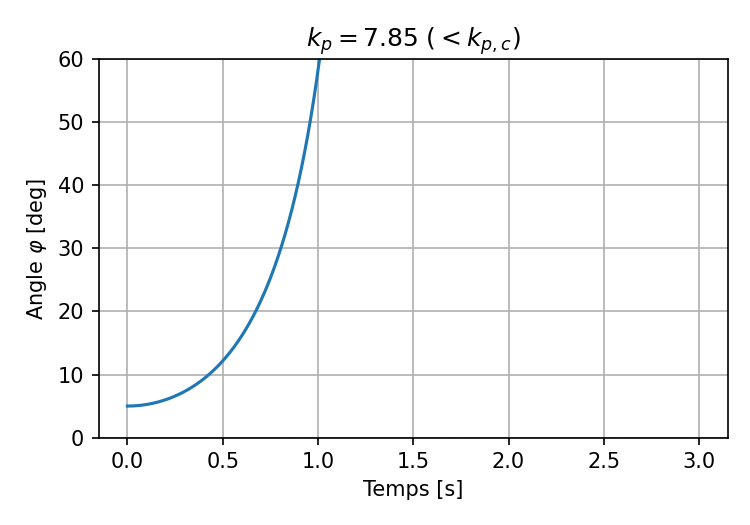
\includegraphics[width=\linewidth]{figures/kp_below.png}
  \end{column}
  \begin{column}{0.48\textwidth}
    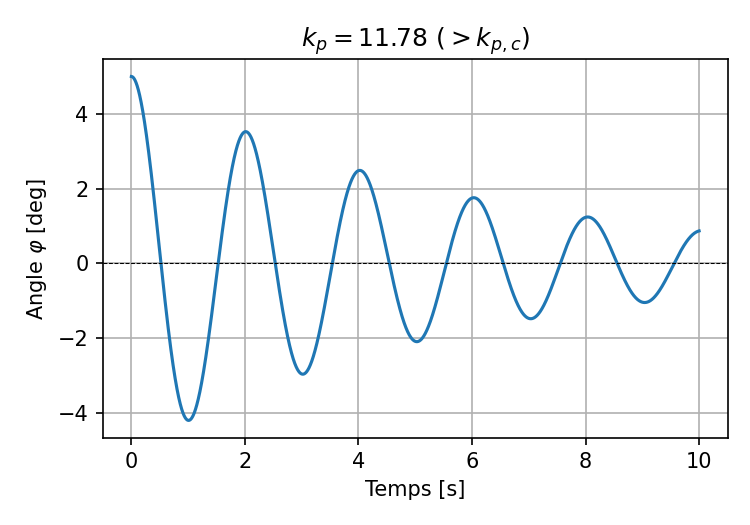
\includegraphics[width=\linewidth]{figures/kp_above.png}
  \end{column}
\end{columns}

\end{frame}

%%%%%%%%%%%%%%%%%%%%%%%%%%%%%%%%%%%%%%%%%%%%%%%%

\begin{frame}
\frametitle{Contrôle PD}
\framesubtitle{Contrôleur Dérivatif}

% Expliquer comment le contrôleur derivatif modifie la dynamique du système: ça ajoute de l'amortissement.
% Ca peut être important pour le confort sur un segway par exemple.

Avec $u = -k_p\,\varphi - k_d\,\dot{\varphi}$, l'équation linéarisée devient :
\[
  D\,\ddot{\varphi} + (c + ml\,k_d)\,\dot{\varphi} + (ml\,k_p - mgl)\,\varphi = 0
\]
Amortissement critique:
\[
  k_{d,c} = \frac{1}{ml}\!\left(2\sqrt{D\,(ml\,k_p - mgl)} - c\right)
\]

\begin{figure}
    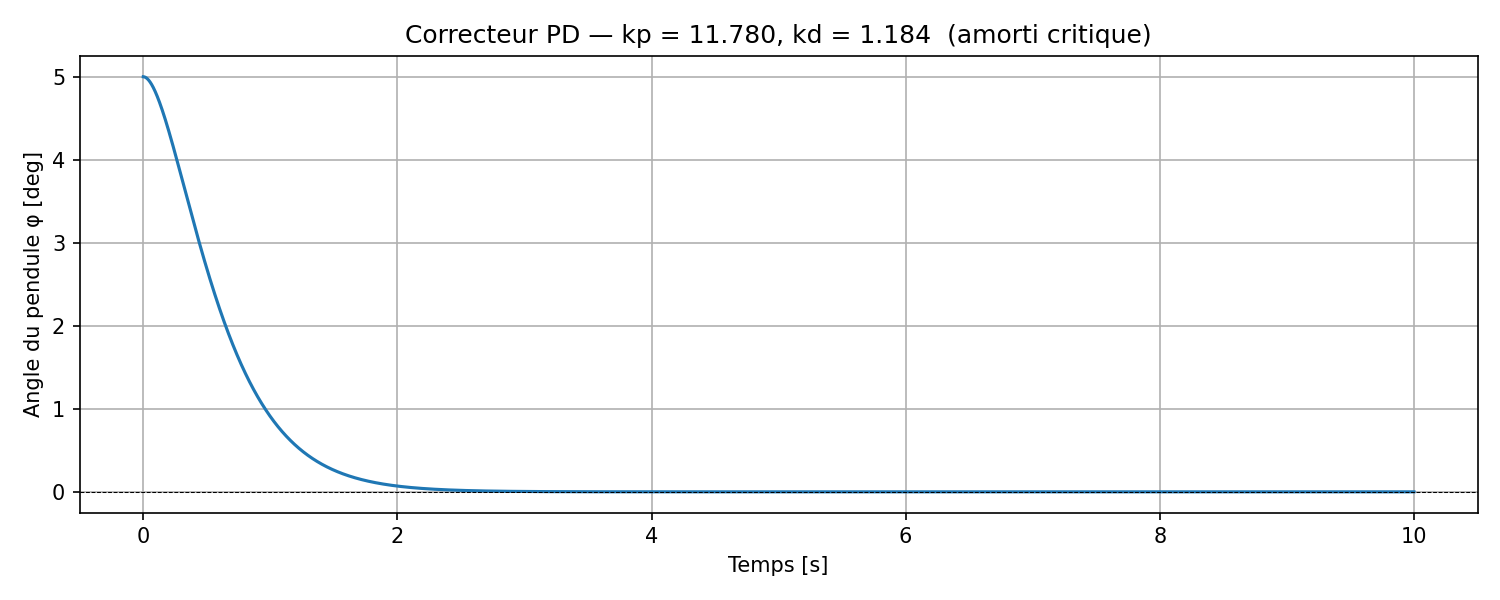
\includegraphics[width=0.8\linewidth]{figures/kp_kd.png}
\end{figure}

\end{frame}

%%%%%%%%%%%%%%%%%%%%%%%%%%%%%%%%%%%%%%%%%%%%%%%%

\begin{frame}
\frametitle{Contrôle PD}
\framesubtitle{Résultats expérimentaux}

\begin{figure}
    \only<1>{%
        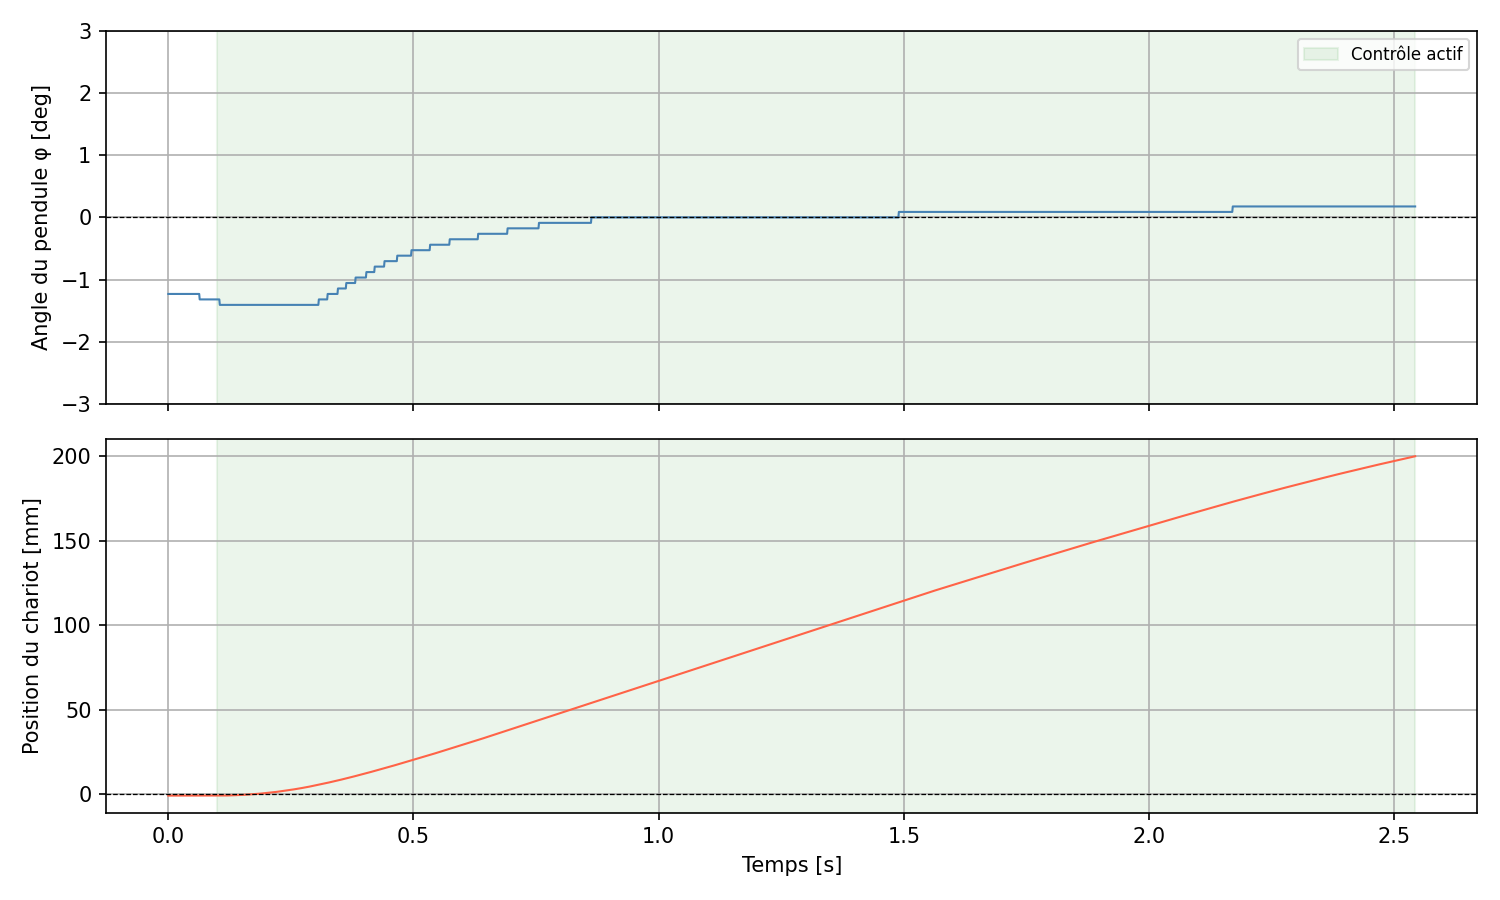
\includegraphics[width=0.85\linewidth]{figures/kp_12_kd_1_stable_bis.png}\\[2pt]
        {\scriptsize Résultats expérimentaux — $k_p = 12$, $k_d = 1$}
    }%
    \only<2>{%
        Même comportement en simulation:
        $\phi$ est correctement stabilisé, mais le chariot n'est pas stable.

        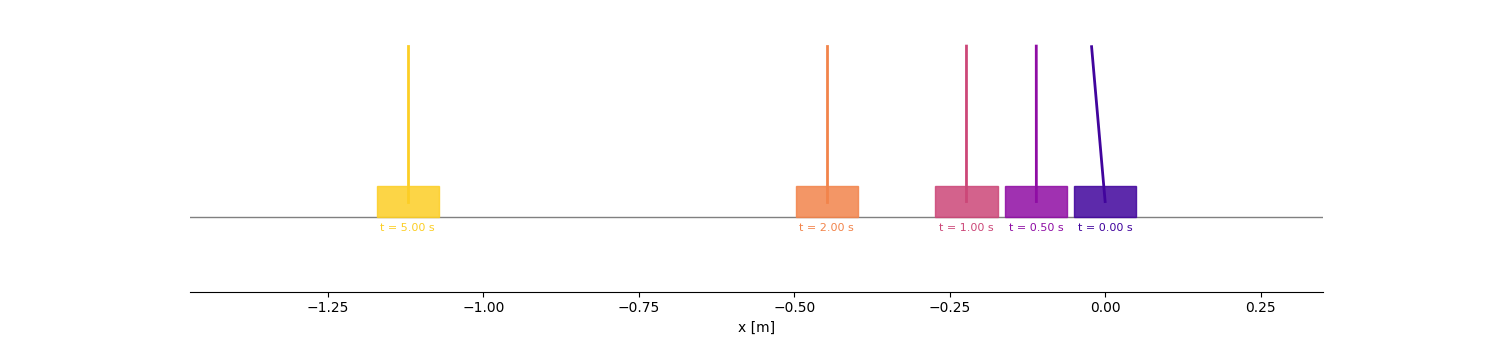
\includegraphics[width=\linewidth]{figures/snapshots_simulation_kp_kd_1.png}\\[2pt]
        {\scriptsize Résultats de simulation — $k_p = 12$, $k_d$}

        \vspace{1em}

        Pour contrôler à la fois $\phi$ et $x$, le contrôleur PD n'est pas adapté.
    }
\end{figure}

\end{frame}


